% !TEX TS-program = pdflatex
% !TEX encoding = UTF-8 Unicode

% This is a simple template for a LaTeX document using the "article" class.
% See "book", "report", "letter" for other types of document.

\documentclass[20pt]{article} % use larger type; default would be 10pt

\usepackage[utf8]{inputenc} % set input encoding (not needed with XeLaTeX)

%%% Examples of Article customizations
% These packages are optional, depending whether you want the features they provide.
% See the LaTeX Companion or other references for full information.

%%% PAGE DIMENSIONS
\usepackage{geometry} % to change the page dimensions
\geometry{a4paper} % or letterpaper (US) or a5paper or....
% \geometry{margin=2in} % for example, change the margins to 2 inches all round
% \geometry{landscape} % set up the page for landscape
%   read geometry.pdf for detailed page layout information

\usepackage{graphicx} % support the \includegraphics command and options

% \usepackage[parfill]{parskip} % Activate to begin paragraphs with an empty line rather than an indent

%%% PACKAGES
\usepackage{booktabs} % for much better looking tables
\usepackage{array} % for better arrays (eg matrices) in maths
\usepackage{paralist} % very flexible & customisable lists (eg. enumerate/itemize, etc.)
\usepackage{verbatim} % adds environment for commenting out blocks of text & for better verbatim
%\usepackage{subfig} % make it possible to include more than one captioned figure/table in a single float
\usepackage{mathtools}
\usepackage{graphicx} % supports images in latex
% These packages are all incorporated in the memoir class to one degree or another...

\usepackage{graphicx}
\usepackage{subcaption}

%%% Other stuff
\DeclarePairedDelimiter\ceil{\lceil}{\rceil}
\DeclarePairedDelimiter\floor{\lfloor}{\rfloor}

%%% HEADERS & FOOTERS
\usepackage{fancyhdr} % This should be set AFTER setting up the page geometry
\pagestyle{fancy} % options: empty , plain , fancy
\renewcommand{\headrulewidth}{0pt} % customise the layout...
\lhead{}\chead{}\rhead{}
\lfoot{}\cfoot{\thepage}\rfoot{}

%%% SECTION TITLE APPEARANCE
\usepackage{sectsty}
\allsectionsfont{\sffamily\mdseries\upshape} % (See the fntguide.pdf for font help)
% (This matches ConTeXt defaults)

%%% ToC (table of contents) APPEARANCE
\usepackage[nottoc,notlof,notlot]{tocbibind} % Put the bibliography in the ToC
\usepackage[titles,subfigure]{tocloft} % Alter the style of the Table of Contents
\renewcommand{\cftsecfont}{\rmfamily\mdseries\upshape}
\renewcommand{\cftsecpagefont}{\rmfamily\mdseries\upshape} % No bold!

%%% graphics path


%%% END Article customizations

%%% nice things to keep around
%\begin{figure}[!htbp]
%  	\centering
%   	\begin{subfigure}[p]{0.5\linewidth}
%    	\includegraphics[width=\linewidth]{}
%   	\end{subfigure}
%\end{figure} 

% \noindent\rule{2cm}{0.4pt} 
%%% puts a small horizontal line

% \mathcal{O} 
%%% big O notation

%%% The "real" document content comes below...

\title{Research Topic Outline}
\author{Liam Dillingham}
%\date{} % Activate to display a given date or no date (if empty),
         % otherwise the current date is printed 

\begin{document}
\maketitle

\section{Abstract}
Although we live in a three-dimensional space, I think it is possible to visualize the 4th dimension using a series of 3-dimensional cross-sections of the fourth dimension.  Using a infinite-book technique, I want to demonstrate how to visualize the fourth dimension, and explore some of the properties that this model may contain, determine if they are beneficial, in hopes that others can use and apply them to aid in understanding their work.

\section{Background}

\section{Proofs/generalization(?)}
\subsection{Generalization}
I want to show how my model of representing the 4th dimension can be generalized from the 0th to the 3rd, and then how it can apply to the 4th dimension
\subsection{relation(?)}
I thought that maybe I can show that my model is consistent with already accepted methods of visualizing higher dimensionality.

\newpage
\section{Illustration}
I plan on having many illustrations throughout the body of the paper, since the purpose of this paper is to visualize, however, I'd like some section reserved to just stepping through the visualization.  I plan on also including some animations I plan on building which I can link to or embed in the paper.

\begin{figure}[h]
\centering
\begin{subfigure}{.5\textwidth}
  \centering
  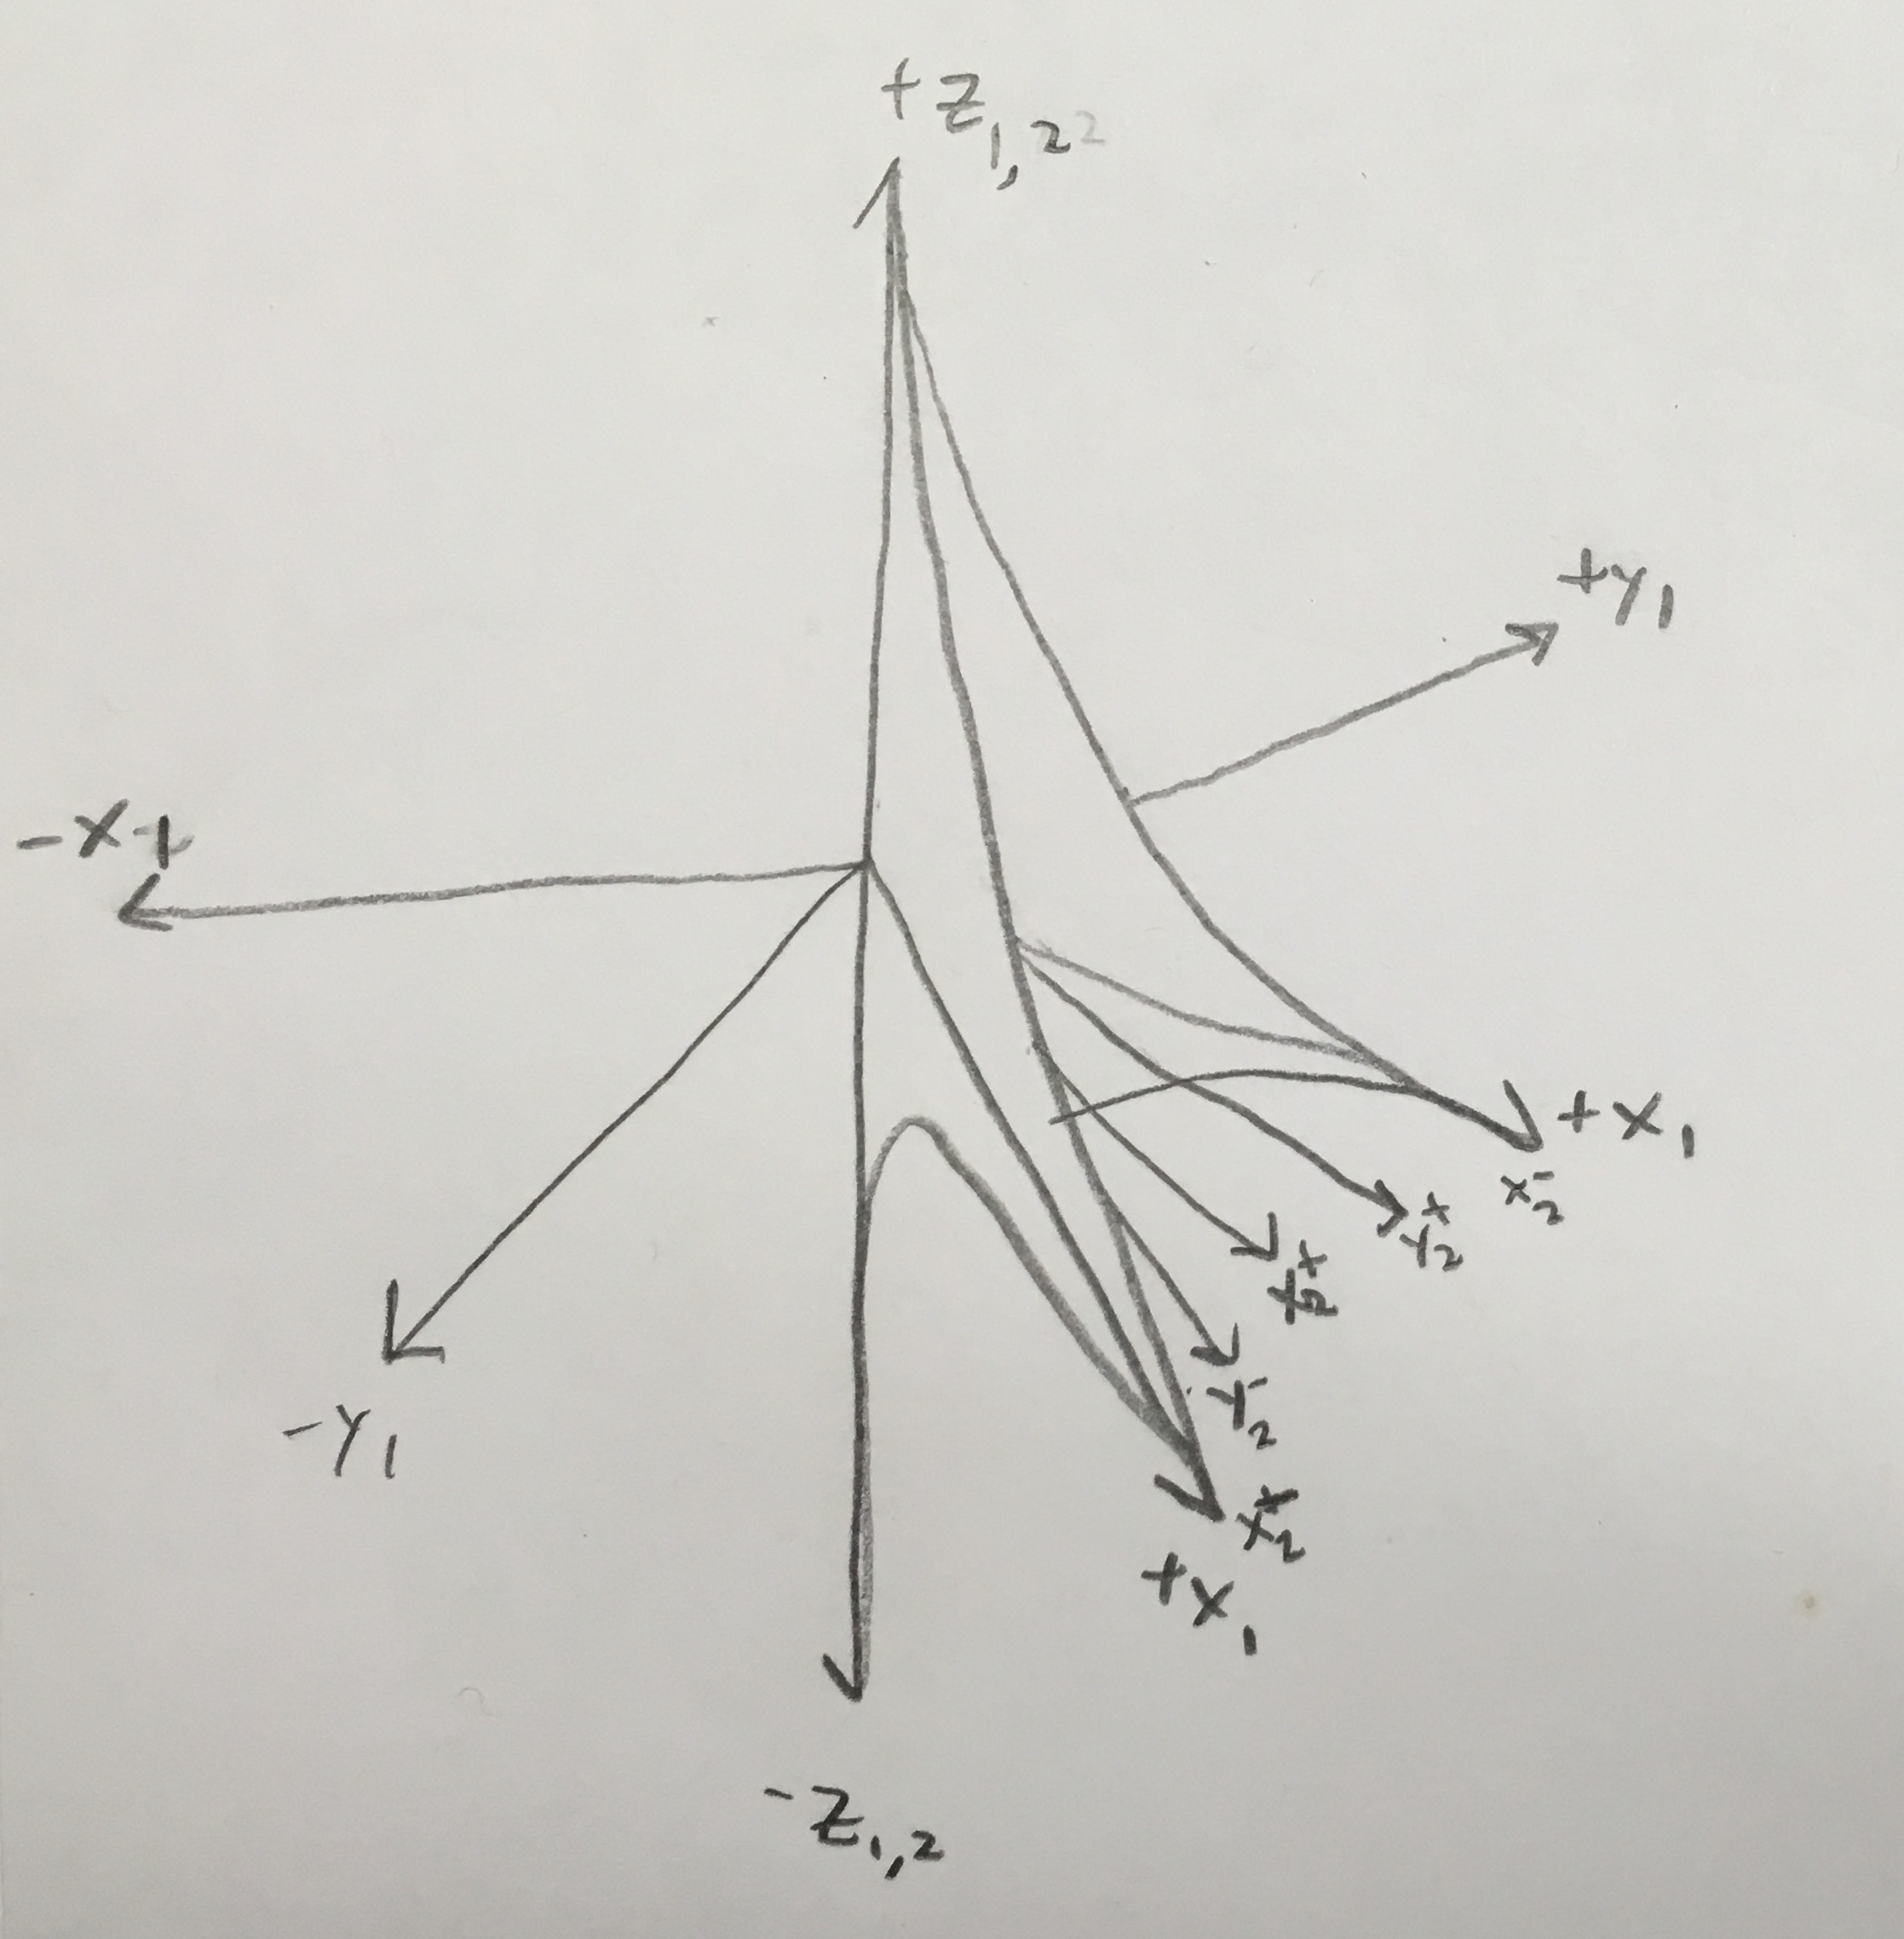
\includegraphics[width=.6\linewidth]{./figures/fig1.jpg}
  \caption{figure 1}
  \label{fig:sub1}
\end{subfigure}%
\begin{subfigure}{.5\textwidth}
  \centering
  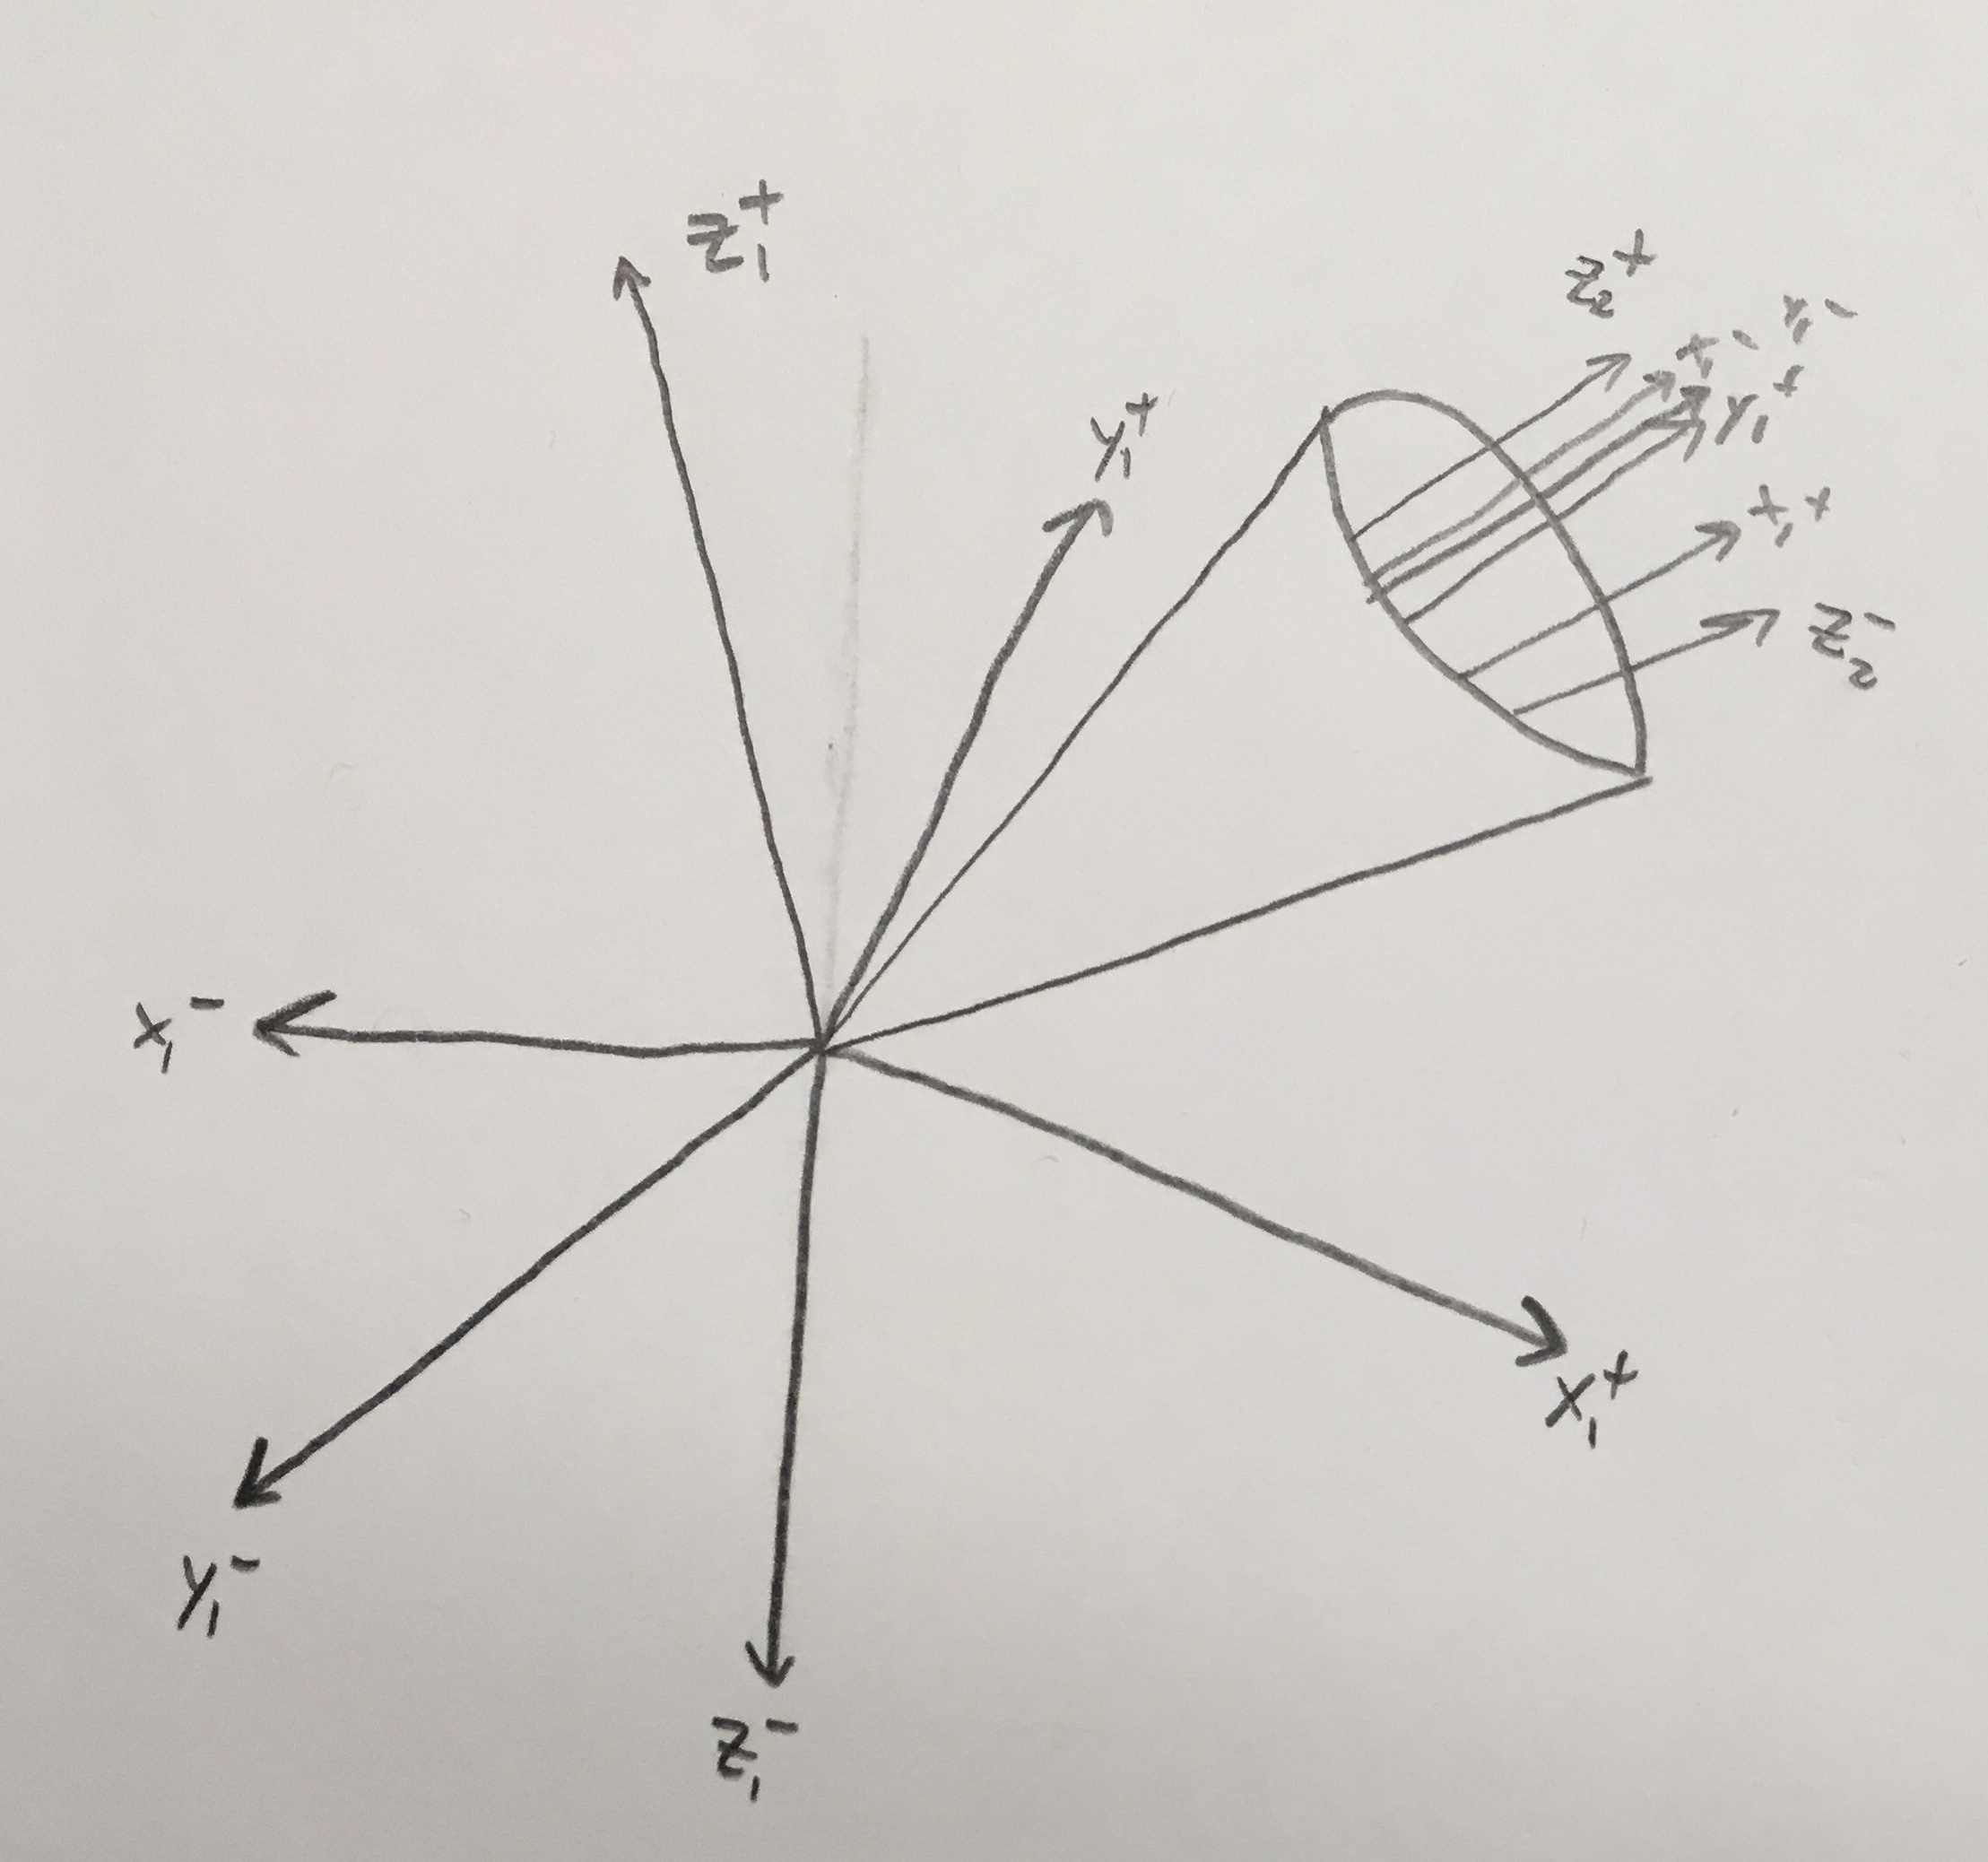
\includegraphics[width=.6\linewidth]{./figures/fig2.jpg}
  \caption{figure 2}
  \label{fig:sub2}
\end{subfigure}
%\caption{A figure with two subfigures}
\label{fig:test}
\end{figure}

\section{Exploration(?)}
Since this is a topic I've come up with myself, I'd like to talk about some of the properties of the model and see if there is anything interesting or of value about them.\\

One example (if you refer to figure 1) you can see that the 3D space consisting of $x_1, y_1, z_1$ and their positive and negative counter parts, takes up a larger proportion of the cross-sectional four-dimensional line segment than the $x_2, y_2, z_2$ 3-space. \\

In addition, if you look at the two figures, they are both attempting to illustrate the same sort of four-dimensional line segment but interpolating in different ways.  In the first one, the two spaces seem to be splitting around the $z$-axis, almost as if the $z$-axis is the spine of a book, and the spaces rotate and fold around it.  In the next one, we have a seemingly arbitrary opening such that the division between the spaces appears as a cone.  Do these differences mean anything? \\

Id also like to talk about objects that pass through multiple 3-dimensional spaces.  If you look at the two figures, each represents a 4-D line segment.  In each of these segments, we see two 3-D points divided by some boundary.  This boundary is of course the "line" part of the segment, and there are infinitely many 3-D spaces folded up between these two points, and you can see that these two 3-D spaces appear to be orthogonal to each other. \\

However, what if we had some object that was able to cross this "boundary"? lets define the 4th axis as the $w$-axis.  If we move along the $w$-axis in the positive direction, then we are increasing time (for simplicity and understanding).  That is, we are iterating through an uncountable number of 3-D spaces.  Suppose a ball is dropped on the ground. As we iterate through our 3-spaces, we can watch the ball move.  Yet we cannot map two 4-D positions into the same 3-D spaces, as the both would be "in two places at the same time".  What happens if there is an object that can cross these boundaries?  Can it exist? \\

I'd like to explore these kinds of questions in my paper.
\end{document}
